\section{Interpretation}
\label{sec:vergleich}
Die Ergebnisse verdeutlichen, dass H2 und H3 bestätigt werden konnten. Die Servicequalität hat einen starken Einfluss auf die Nutzerzufriedenheit, während die Nutzerzufriedenheit wiederum einen starken Einfluss auf den Net Benefit hat. Die Systemqualität konnte dagegen kein signifikanter Einfluss auf die Nutzerzufriedenheit attestiert werden.  
\todo consistency at large. 
Hohe Dropout Raten bei MOOCS. Besonderheiten von MOOC auflisten: 


The story of MOOCs is not going to be told with conventional statistics borrowed from brick-and-mortar classroom models. Rather, our research describes an emerging learning ecosystem, one where enrollment can be casual and nonbinding, learning happens asynchronously, and registrants come from all countries in the world, with diverse intentions and patterns of learning. The metrics we choose should respect their intentions and encourage their learning.\parencite{reich2014tricky}


\begin{figure}[h]
\centering
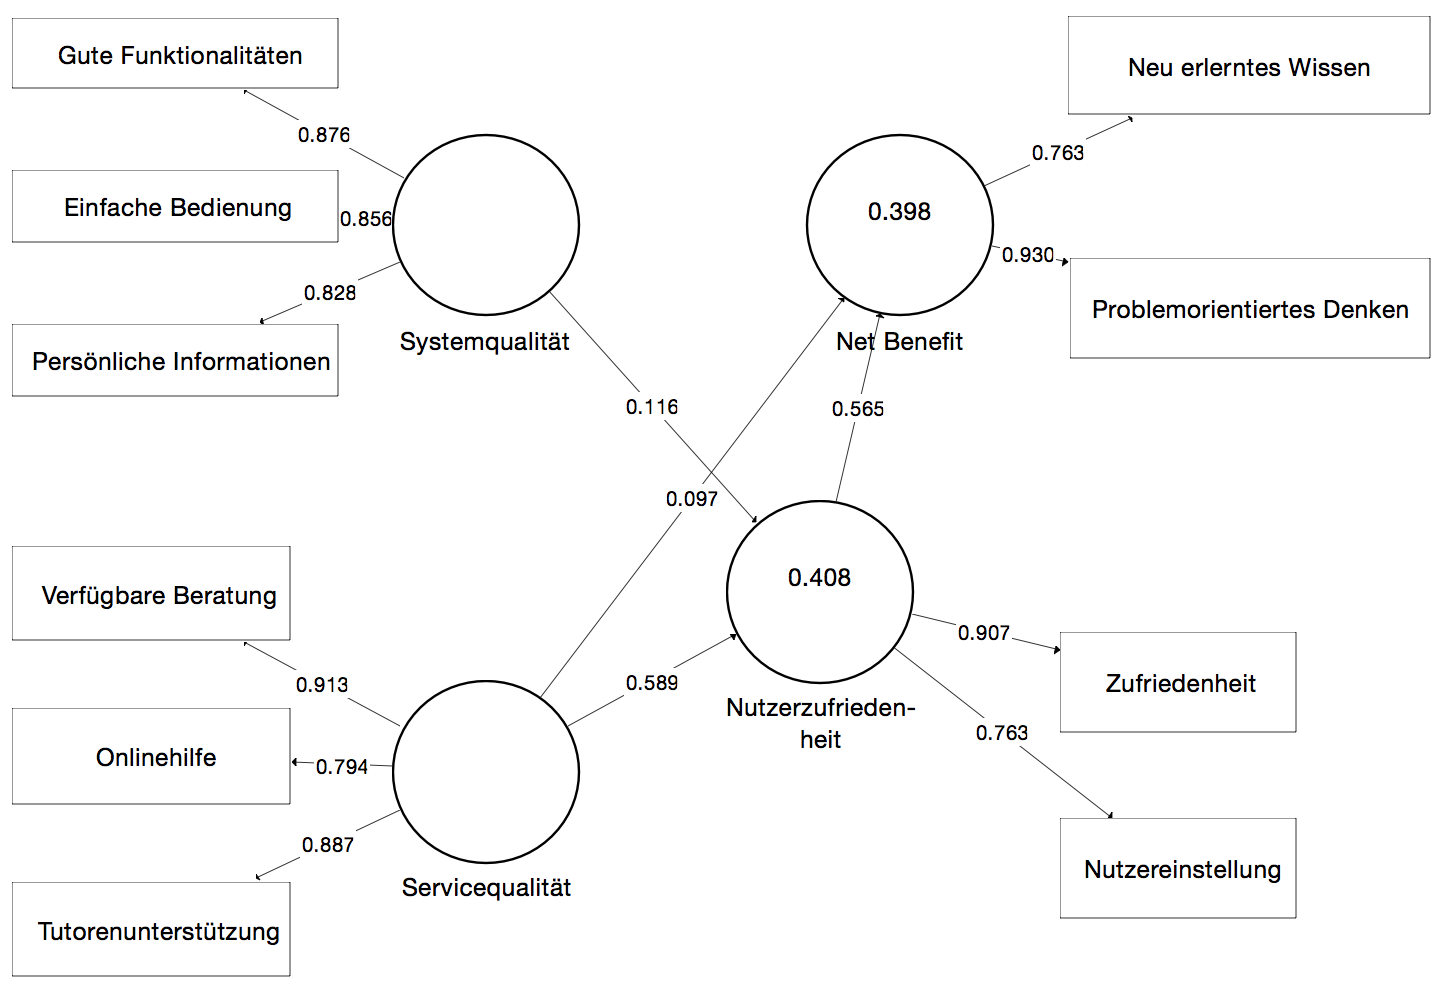
\includegraphics[width=1\textwidth]{Grafiken/pls_bw_3.png}
\caption{PLS Modellergebnisse}
\label{PLS Modellergebnisse}
\end{figure}